\documentclass[landscape]{article}
\setlength\textwidth{10in}
\setlength\textheight{8.5in}
\setlength\oddsidemargin{-.5in}
\setlength\evensidemargin{-.5in}
\setlength\topmargin{-.7in}
\setlength\headsep{0in}
\setlength\headheight{0in}
\setlength\topskip{0in}
\usepackage{tikz-qtree-compat}
\usepackage{spverbatim}
\usepackage{amssymb}
\usepackage{rotating}
\usepackage{color}
\usepackage{environ}
\usepackage{graphicx}
\usepackage{calc}

\newlength{\xsize}
\newlength{\ysize}
\newsavebox{\tempbox}

\newcommand{\maxsize}[1]{
  \savebox{\tempbox}{#1}
  \settoheight{\ysize}{\usebox{\tempbox}}
  \settowidth{\xsize}{\usebox{\tempbox}}
  \pgfmathparse{\xsize/\textwidth > \ysize/\textheight}
  \if \pgfmathresult1
    \resizebox{\textwidth}{!}{\usebox{\tempbox}}
  \else
    \resizebox{!}{\textheight-2cm}{\usebox{\tempbox}}
  \fi
}

\begin{document}
  \begin{spverbatim}
    4835 (5397, p, no): A man is removing some food from a box
  \end{spverbatim}
  \noindent\maxsize{\begin{tikzpicture}[grow=down]
    \tikzset{level distance = 25pt, sibling distance = 0pt}
    \tikzset{every tree node/.style={align=center,anchor=north}}
    \Tree
      [.\node{${\tt ba}[s\!:\!dcl]$};
       [.\node{${\tt fa}[np]$};
        [.\node{
        \texttt{A}\\
        $np/n$\\
        \textbf{a}\\
        \normalsize{DT}\\
        \scriptsize{I-NP}\\
        \scriptsize{O} };
        ]
        [.\node{
        \texttt{man}\\
        $n$\\
        \textbf{man}\\
        \normalsize{NN}\\
        \scriptsize{I-NP}\\
        \scriptsize{O} };
        ]
       ]
       [.\node{${\tt fa}[s\!:\!dcl\backslash np]$};
        [.\node{
        \texttt{is}\\
        $(s\!:\!dcl\backslash np)/ (s\!:\!ng\backslash np)$\\
        \textbf{be}\\
        \normalsize{VBZ}\\
        \scriptsize{I-VP}\\
        \scriptsize{O} };
        ]
        [.\node{${\tt fa}[s\!:\!ng\backslash np]$};
         [.\node{${\tt fa}[(s\!:\!ng\backslash np)/pp]$};
          [.\node{
          \texttt{removing}\\
          $((s\!:\!ng\backslash np)/pp)/np$\\
          \textbf{remove}\\
          \normalsize{VBG}\\
          \scriptsize{I-VP}\\
          \scriptsize{O} };
          ]
          [.\node{${\tt fa}[np]$};
           [.\node{
           \texttt{some}\\
           $np/n$\\
           \textbf{some}\\
           \normalsize{DT}\\
           \scriptsize{I-NP}\\
           \scriptsize{O} };
           ]
           [.\node{
           \texttt{food}\\
           $n$\\
           \textbf{food}\\
           \normalsize{NN}\\
           \scriptsize{I-NP}\\
           \scriptsize{O} };
           ]
          ]
         ]
         [.\node{${\tt fa}[pp]$};
          [.\node{
          \texttt{from}\\
          $pp/np$\\
          \textbf{from}\\
          \normalsize{IN}\\
          \scriptsize{I-PP}\\
          \scriptsize{O} };
          ]
          [.\node{${\tt fa}[np]$};
           [.\node{
           \texttt{a}\\
           $np/n$\\
           \textbf{a}\\
           \normalsize{DT}\\
           \scriptsize{I-NP}\\
           \scriptsize{O} };
           ]
           [.\node{
           \texttt{box}\\
           $n$\\
           \textbf{box}\\
           \normalsize{NN}\\
           \scriptsize{I-NP}\\
           \scriptsize{O} };
           ]
          ]
         ]
        ]
       ]
      ]
  \end{tikzpicture}
  }
  \clearpage
\noindent\maxsize{
\begin{tikzpicture}[grow=down]
\tikzset{level distance = 25pt, sibling distance = -5pt}
\tikzset{every tree node/.style={align=center,anchor=north}}
\Tree
  [.\node{$s_{dcl}$};
   [.\node{$np,s_{dcl}$};
    [.\node{
    \texttt{is}\\
    $(np,s_{ng}),np,s_{dcl}$\\
    \textbf{be}\\
    \normalsize{VBZ}\\
    \scriptsize{I-VP}\\
    \scriptsize{O} };
    ]
    [.\node{$np,s_{ng}$};
     [.\node{$pp,np,s_{ng}$};
      [.\node{
      \texttt{removing}\\
      $np,pp,np,s_{ng}$\\
      \textbf{remove}\\
      \normalsize{VBG}\\
      \scriptsize{I-VP}\\
      \scriptsize{O} };
      ]
      [.\node{$np$};
       [.\node{
       \texttt{some}\\
       $n,np$\\
       \textbf{some}\\
       \normalsize{DT}\\
       \scriptsize{I-NP}\\
       \scriptsize{O} };
       ]
       [.\node{
       \texttt{food}\\
       $n$\\
       \textbf{food}\\
       \normalsize{NN}\\
       \scriptsize{I-NP}\\
       \scriptsize{O} };
       ]
      ]
     ]
     [.\node{$pp$};
      [.\node{
      \texttt{from}\\
      $np,pp$\\
      \textbf{from}\\
      \normalsize{IN}\\
      \scriptsize{I-PP}\\
      \scriptsize{O} };
      ]
      [.\node{$np$};
       [.\node{
       \texttt{a}\\
       $n,np$\\
       \textbf{a}\\
       \normalsize{DT}\\
       \scriptsize{I-NP}\\
       \scriptsize{O} };
       ]
       [.\node{
       \texttt{box}\\
       $n$\\
       \textbf{box}\\
       \normalsize{NN}\\
       \scriptsize{I-NP}\\
       \scriptsize{O} };
       ]
      ]
     ]
    ]
   ]
   [.\node{$np$};
    [.\node{
    \texttt{A}\\
    $n,np$\\
    \textbf{a}\\
    \normalsize{DT}\\
    \scriptsize{I-NP}\\
    \scriptsize{O} };
    ]
    [.\node{
    \texttt{man}\\
    $n$\\
    \textbf{man}\\
    \normalsize{NN}\\
    \scriptsize{I-NP}\\
    \scriptsize{O} };
    ]
   ]
  ]
\end{tikzpicture}
}
\clearpage
\noindent\maxsize{
\begin{tikzpicture}[grow=down]
\tikzset{level distance = 25pt, sibling distance = -5pt}
\tikzset{every tree node/.style={align=center,anchor=north}}
\Tree
  [.\node{$s_{dcl}$};
   [.\node{$np,s_{dcl}$};
    [.\node{
    \texttt{is}\\
    $(np,s_{ng}),np,s_{dcl}$\\
    \textbf{be}\\
    \normalsize{VBZ}\\
    \scriptsize{I-VP}\\
    \scriptsize{O} };
    ]
    [.\node{$np,s_{ng}$};
     [.\node{$pp,np,s_{ng}$};
      [.\node{
      \texttt{removing}\\
      $np,pp,np,s_{ng}$\\
      \textbf{remove}\\
      \normalsize{VBG}\\
      \scriptsize{I-VP}\\
      \scriptsize{O} };
      ]
      [.\node{$np$};
       [.\node{
       \texttt{some}\\
       $n,np$\\
       \textbf{a}\\
       \normalsize{DT}\\
       \scriptsize{I-NP}\\
       \scriptsize{O} };
       ]
       [.\node{
       \texttt{food}\\
       $n$\\
       \textbf{food}\\
       \normalsize{NN}\\
       \scriptsize{I-NP}\\
       \scriptsize{O} };
       ]
      ]
     ]
     [.\node{$pp$};
      [.\node{
      \texttt{from}\\
      $np,pp$\\
      \textbf{from}\\
      \normalsize{IN}\\
      \scriptsize{I-PP}\\
      \scriptsize{O} };
      ]
      [.\node{$np$};
       [.\node{
       \texttt{a}\\
       $n,np$\\
       \textbf{a}\\
       \normalsize{DT}\\
       \scriptsize{I-NP}\\
       \scriptsize{O} };
       ]
       [.\node{
       \texttt{box}\\
       $n$\\
       \textbf{box}\\
       \normalsize{NN}\\
       \scriptsize{I-NP}\\
       \scriptsize{O} };
       ]
      ]
     ]
    ]
   ]
   [.\node{$np$};
    [.\node{
    \texttt{A}\\
    $n,np$\\
    \textbf{a}\\
    \normalsize{DT}\\
    \scriptsize{I-NP}\\
    \scriptsize{O} };
    ]
    [.\node{
    \texttt{man}\\
    $n$\\
    \textbf{man}\\
    \normalsize{NN}\\
    \scriptsize{I-NP}\\
    \scriptsize{O} };
    ]
   ]
  ]
\end{tikzpicture}
}
\clearpage
a man (be $(\lambda X_{9996}$.a box $(\lambda X_{9545}$.a food $(\lambda X_{9471}$.remove $X_{9471}$ (from $X_{9545}$) $X_{9996}$))))


\noindent\maxsize{
\begin{tikzpicture}[grow=down]
\tikzset{level distance = 25pt, sibling distance = -5pt}
\tikzset{every tree node/.style={align=center,anchor=north}}
\Tree
      [.\node{$s_{dcl}$};
       [.\node{$(np,s_{dcl}),s_{dcl}$};
        [.\node{
        \texttt{A}\\
        $n,(np,s_{dcl}),s_{dcl}$\\
        \textbf{a}\\
        \normalsize{DT}\\
        \scriptsize{I-NP}\\
        \scriptsize{O} };
        ]
        [.\node{
        \texttt{man}\\
        $n$\\
        \textbf{man}\\
        \normalsize{NN}\\
        \scriptsize{I-NP}\\
        \scriptsize{O} };
        ]
       ]
       [.\node{$np,s_{dcl}$};
        [.\node{
        \texttt{is}\\
        $(np,s_{ng}),np,s_{dcl}$\\
        \textbf{be}\\
        \normalsize{VBZ}\\
        \scriptsize{I-VP}\\
        \scriptsize{O} };
        ]
        [.\node{$np,s_{ng}$};
         [.\node{              \textbf{$\lambda X_{9996}$}\\
              $np$
             };
         ]
         [.\node{$s_{ng}$};
          [.\node{$(np,s_{ng}),s_{ng}$};
           [.\node{
           \texttt{a}\\
           $n,(np,s_{ng}),s_{ng}$\\
           \textbf{a}\\
           \normalsize{DT}\\
           \scriptsize{I-NP}\\
           \scriptsize{O} };
           ]
           [.\node{
           \texttt{box}\\
           $n$\\
           \textbf{box}\\
           \normalsize{NN}\\
           \scriptsize{I-NP}\\
           \scriptsize{O} };
           ]
          ]
          [.\node{$np,s_{ng}$};
           [.\node{                \textbf{$\lambda X_{1091}$}\\
                $np$
               };
           ]
           [.\node{$s_{ng}$};
            [.\node{$(np,s_{ng}),s_{ng}$};
             [.\node{
             \texttt{some}\\
             $n,(np,s_{ng}),s_{ng}$\\
             \textbf{a}\\
             \normalsize{DT}\\
             \scriptsize{I-NP}\\
             \scriptsize{O} };
             ]
             [.\node{
             \texttt{food}\\
             $n$\\
             \textbf{food}\\
             \normalsize{NN}\\
             \scriptsize{I-NP}\\
             \scriptsize{O} };
             ]
            ]
            [.\node{$np,s_{ng}$};
             [.\node{                  \textbf{$\lambda X_{1090}$}\\
                  $np$
                 };
             ]
             [.\node{$s_{ng}$};
              [.\node{$np,s_{ng}$};
               [.\node{$pp,np,s_{ng}$};
                [.\node{
                \texttt{removing}\\
                $np,pp,np,s_{ng}$\\
                \textbf{remove}\\
                \normalsize{VBG}\\
                \scriptsize{I-VP}\\
                \scriptsize{O} };
                ]
                [.\node{                     \textbf{$X_{1090}$}\\
                     $np$
                    };
                ]
               ]
               [.\node{$pp$};
                [.\node{
                \texttt{from}\\
                $np,pp$\\
                \textbf{from}\\
                \normalsize{IN}\\
                \scriptsize{I-PP}\\
                \scriptsize{O} };
                ]
                [.\node{                     \textbf{$X_{1091}$}\\
                     $np$
                    };
                ]
               ]
              ]
              [.\node{                   \textbf{$X_{1131}$}\\
                   $np$
                  };
              ]
             ]
            ]
           ]
          ]
         ]
        ]
       ]
      ]
\end{tikzpicture}
}
\clearpage
  \begin{spverbatim}
    4836 (5397, h, no): The man is putting chicken into the container
  \end{spverbatim}
  \noindent\maxsize{\begin{tikzpicture}[grow=down]
    \tikzset{level distance = 25pt, sibling distance = 0pt}
    \tikzset{every tree node/.style={align=center,anchor=north}}
    \Tree
      [.\node{${\tt ba}[s\!:\!dcl]$};
       [.\node{${\tt fa}[np]$};
        [.\node{
        \texttt{The}\\
        $np/n$\\
        \textbf{the}\\
        \normalsize{DT}\\
        \scriptsize{I-NP}\\
        \scriptsize{O} };
        ]
        [.\node{
        \texttt{man}\\
        $n$\\
        \textbf{man}\\
        \normalsize{NN}\\
        \scriptsize{I-NP}\\
        \scriptsize{O} };
        ]
       ]
       [.\node{${\tt fa}[s\!:\!dcl\backslash np]$};
        [.\node{
        \texttt{is}\\
        $(s\!:\!dcl\backslash np)/ (s\!:\!ng\backslash np)$\\
        \textbf{be}\\
        \normalsize{VBZ}\\
        \scriptsize{I-VP}\\
        \scriptsize{O} };
        ]
        [.\node{${\tt fa}[s\!:\!ng\backslash np]$};
         [.\node{${\tt fa}[(s\!:\!ng\backslash np)/pp]$};
          [.\node{
          \texttt{putting}\\
          $((s\!:\!ng\backslash np)/pp)/np$\\
          \textbf{put}\\
          \normalsize{VBG}\\
          \scriptsize{I-VP}\\
          \scriptsize{O} };
          ]
          [.\node{${\tt lx}[np, n]$};
           [.\node{
           \texttt{chicken}\\
           $n$\\
           \textbf{chicken}\\
           \normalsize{NN}\\
           \scriptsize{I-NP}\\
           \scriptsize{O} };
           ]
          ]
         ]
         [.\node{${\tt fa}[pp]$};
          [.\node{
          \texttt{into}\\
          $pp/np$\\
          \textbf{into}\\
          \normalsize{IN}\\
          \scriptsize{I-PP}\\
          \scriptsize{O} };
          ]
          [.\node{${\tt fa}[np]$};
           [.\node{
           \texttt{the}\\
           $np/n$\\
           \textbf{the}\\
           \normalsize{DT}\\
           \scriptsize{I-NP}\\
           \scriptsize{O} };
           ]
           [.\node{
           \texttt{container}\\
           $n$\\
           \textbf{container}\\
           \normalsize{NN}\\
           \scriptsize{I-NP}\\
           \scriptsize{O} };
           ]
          ]
         ]
        ]
       ]
      ]
  \end{tikzpicture}
  }
  \clearpage
\noindent\maxsize{
\begin{tikzpicture}[grow=down]
\tikzset{level distance = 25pt, sibling distance = -5pt}
\tikzset{every tree node/.style={align=center,anchor=north}}
\Tree
  [.\node{$s_{dcl}$};
   [.\node{$np,s_{dcl}$};
    [.\node{
    \texttt{is}\\
    $(np,s_{ng}),np,s_{dcl}$\\
    \textbf{be}\\
    \normalsize{VBZ}\\
    \scriptsize{I-VP}\\
    \scriptsize{O} };
    ]
    [.\node{$np,s_{ng}$};
     [.\node{$pp,np,s_{ng}$};
      [.\node{
      \texttt{putting}\\
      $np,pp,np,s_{ng}$\\
      \textbf{put}\\
      \normalsize{VBG}\\
      \scriptsize{I-VP}\\
      \scriptsize{O} };
      ]
      [.\node{$np$};
       [.\node{
       \texttt{chicken}\\
       $n$\\
       \textbf{chicken}\\
       \normalsize{NN}\\
       \scriptsize{I-NP}\\
       \scriptsize{O} };
       ]
      ]
     ]
     [.\node{$pp$};
      [.\node{
      \texttt{into}\\
      $np,pp$\\
      \textbf{into}\\
      \normalsize{IN}\\
      \scriptsize{I-PP}\\
      \scriptsize{O} };
      ]
      [.\node{$np$};
       [.\node{
       \texttt{the}\\
       $n,np$\\
       \textbf{the}\\
       \normalsize{DT}\\
       \scriptsize{I-NP}\\
       \scriptsize{O} };
       ]
       [.\node{
       \texttt{container}\\
       $n$\\
       \textbf{container}\\
       \normalsize{NN}\\
       \scriptsize{I-NP}\\
       \scriptsize{O} };
       ]
      ]
     ]
    ]
   ]
   [.\node{$np$};
    [.\node{
    \texttt{The}\\
    $n,np$\\
    \textbf{the}\\
    \normalsize{DT}\\
    \scriptsize{I-NP}\\
    \scriptsize{O} };
    ]
    [.\node{
    \texttt{man}\\
    $n$\\
    \textbf{man}\\
    \normalsize{NN}\\
    \scriptsize{I-NP}\\
    \scriptsize{O} };
    ]
   ]
  ]
\end{tikzpicture}
}
\clearpage
\noindent\maxsize{
\begin{tikzpicture}[grow=down]
\tikzset{level distance = 25pt, sibling distance = -5pt}
\tikzset{every tree node/.style={align=center,anchor=north}}
\Tree
  [.\node{$s_{dcl}$};
   [.\node{$np,s_{dcl}$};
    [.\node{
    \texttt{is}\\
    $(np,s_{ng}),np,s_{dcl}$\\
    \textbf{be}\\
    \normalsize{VBZ}\\
    \scriptsize{I-VP}\\
    \scriptsize{O} };
    ]
    [.\node{$np,s_{ng}$};
     [.\node{$pp,np,s_{ng}$};
      [.\node{
      \texttt{putting}\\
      $np,pp,np,s_{ng}$\\
      \textbf{put}\\
      \normalsize{VBG}\\
      \scriptsize{I-VP}\\
      \scriptsize{O} };
      ]
      [.\node{$np$};
       [.\node[text=green]{
       \texttt{a}\\
       $n,np$\\
       \textbf{a}\\
       \normalsize{DT}\\
       \scriptsize{I-NP}\\
       \scriptsize{Ins} };
       ]
       [.\node{
       \texttt{chicken}\\
       $n$\\
       \textbf{chicken}\\
       \normalsize{NN}\\
       \scriptsize{I-NP}\\
       \scriptsize{O} };
       ]
      ]
     ]
     [.\node{$pp$};
      [.\node{
      \texttt{into}\\
      $np,pp$\\
      \textbf{into}\\
      \normalsize{IN}\\
      \scriptsize{I-PP}\\
      \scriptsize{O} };
      ]
      [.\node{$np$};
       [.\node{
       \texttt{the}\\
       $n,np$\\
       \textbf{the}\\
       \normalsize{DT}\\
       \scriptsize{I-NP}\\
       \scriptsize{O} };
       ]
       [.\node{
       \texttt{container}\\
       $n$\\
       \textbf{container}\\
       \normalsize{NN}\\
       \scriptsize{I-NP}\\
       \scriptsize{O} };
       ]
      ]
     ]
    ]
   ]
   [.\node{$np$};
    [.\node{
    \texttt{The}\\
    $n,np$\\
    \textbf{the}\\
    \normalsize{DT}\\
    \scriptsize{I-NP}\\
    \scriptsize{O} };
    ]
    [.\node{
    \texttt{man}\\
    $n$\\
    \textbf{man}\\
    \normalsize{NN}\\
    \scriptsize{I-NP}\\
    \scriptsize{O} };
    ]
   ]
  ]
\end{tikzpicture}
}
\clearpage
the man (be $(\lambda X_{10264}$.the container $(\lambda X_{9813}$.a chicken $(\lambda X_{9739}$.put $X_{9739}$ (into $X_{9813}$) $X_{10264}$))))


\noindent\maxsize{
\begin{tikzpicture}[grow=down]
\tikzset{level distance = 25pt, sibling distance = -5pt}
\tikzset{every tree node/.style={align=center,anchor=north}}
\Tree
      [.\node{$s_{dcl}$};
       [.\node{$(np,s_{dcl}),s_{dcl}$};
        [.\node{
        \texttt{The}\\
        $n,(np,s_{dcl}),s_{dcl}$\\
        \textbf{the}\\
        \normalsize{DT}\\
        \scriptsize{I-NP}\\
        \scriptsize{O} };
        ]
        [.\node{
        \texttt{man}\\
        $n$\\
        \textbf{man}\\
        \normalsize{NN}\\
        \scriptsize{I-NP}\\
        \scriptsize{O} };
        ]
       ]
       [.\node{$np,s_{dcl}$};
        [.\node{
        \texttt{is}\\
        $(np,s_{ng}),np,s_{dcl}$\\
        \textbf{be}\\
        \normalsize{VBZ}\\
        \scriptsize{I-VP}\\
        \scriptsize{O} };
        ]
        [.\node{$np,s_{ng}$};
         [.\node{              \textbf{$\lambda X_{10264}$}\\
              $np$
             };
         ]
         [.\node{$s_{ng}$};
          [.\node{$(np,s_{ng}),s_{ng}$};
           [.\node{
           \texttt{the}\\
           $n,(np,s_{ng}),s_{ng}$\\
           \textbf{the}\\
           \normalsize{DT}\\
           \scriptsize{I-NP}\\
           \scriptsize{O} };
           ]
           [.\node{
           \texttt{container}\\
           $n$\\
           \textbf{container}\\
           \normalsize{NN}\\
           \scriptsize{I-NP}\\
           \scriptsize{O} };
           ]
          ]
          [.\node{$np,s_{ng}$};
           [.\node{                \textbf{$\lambda X_{1322}$}\\
                $np$
               };
           ]
           [.\node{$s_{ng}$};
            [.\node{$(np,s_{ng}),s_{ng}$};
             [.\node[text=green]{
             \texttt{a}\\
             $n,(np,s_{ng}),s_{ng}$\\
             \textbf{a}\\
             \normalsize{DT}\\
             \scriptsize{I-NP}\\
             \scriptsize{Ins} };
             ]
             [.\node{
             \texttt{chicken}\\
             $n$\\
             \textbf{chicken}\\
             \normalsize{NN}\\
             \scriptsize{I-NP}\\
             \scriptsize{O} };
             ]
            ]
            [.\node{$np,s_{ng}$};
             [.\node{                  \textbf{$\lambda X_{1321}$}\\
                  $np$
                 };
             ]
             [.\node{$s_{ng}$};
              [.\node{$np,s_{ng}$};
               [.\node{$pp,np,s_{ng}$};
                [.\node{
                \texttt{putting}\\
                $np,pp,np,s_{ng}$\\
                \textbf{put}\\
                \normalsize{VBG}\\
                \scriptsize{I-VP}\\
                \scriptsize{O} };
                ]
                [.\node{                     \textbf{$X_{1321}$}\\
                     $np$
                    };
                ]
               ]
               [.\node{$pp$};
                [.\node{
                \texttt{into}\\
                $np,pp$\\
                \textbf{into}\\
                \normalsize{IN}\\
                \scriptsize{I-PP}\\
                \scriptsize{O} };
                ]
                [.\node{                     \textbf{$X_{1322}$}\\
                     $np$
                    };
                ]
               ]
              ]
              [.\node{                   \textbf{$X_{1362}$}\\
                   $np$
                  };
              ]
             ]
            ]
           ]
          ]
         ]
        ]
       ]
      ]
\end{tikzpicture}
}
\clearpage
\end{document}